\documentclass[a4paper, 10pt, final, garamond]{book}
\usepackage{cours-preambule}
\graphicspath{{./figures/}}
\addto\captionsfrench{\renewcommand{\figurename}{Fig.}}

\makeatletter
\renewcommand{\@chapapp}{Contrôle de connaissances}
\makeatother

% \toggletrue{student}
% \toggletrue{corrige}
\renewcommand{\mycol}{black}
% \renewcommand{\mycol}{gray}

\begin{document}
\setcounter{chapter}{9}

\settype{enon}
\settype{solu}

\chapter{Électrocinétique en RSF\ifstudent{~(15')}}

\begin{enumerate}[label=\sqenumi]
	\item[n]{5}%
	      Sous quelle forme mathématique s'exprime le signal d'un système en RSF~?
	      Présenter alors le passage en complexes et l'intérêt de cette forme pour
	      la dérivation et l'intégration.
	      \smallbreak
	      \begin{isd}
		      \vspace{-15pt}
		      \psw{%
			      \begin{DispWithArrows*}[groups]
				      y(t) &\stm{=} Y_0 \cos(\wt+\f)
				      % \Arrow{Passage $\Cb$}
				      \\\Lra
				      \yu(t) &\stm{=} Y_0 \exr^{\jj (\wt+\f)}
				      % \Arrow{Séparation de $t$}
				      % \\\Lra
				      % \yu(t) &= \underbracket[1pt]{Y_0\exr^{\jj
				      % \f}}_{=\cte}\cdot\exr^{\jwt}
				      % \Arrow{Réécriture}
				      \\\Lra
				      \Aboxed{\yu(t) &\stm{=} \Yu\exr^{\jwt}}
				      \quad \text{avec} \quad
				      \boxed{\Yu = Y_0\exr^{\jj \f}}
				      % \Ra
				      % \left\{
				      % \begin{array}{ll}
				      % Y_0 & = \abs{\Yu}
				      % \\
				      % \f & = \arg*{\Yu}
				      % \end{array}
				      % \right.
			      \end{DispWithArrows*}
		      }%
		      \vspace{-15pt}
		      \tcblower
		      \psw{%
			      \begin{gather*}
				      \dv{\yu}{t} = \dv{\Yu\exr^{\jwt}}{t} = \jw \cdot \Yu\exr^{\jwt}
				      \Lra
				      \boxed{\dv{\yu}{t} \stm{=} \jw \yu(t)}
				      \\
				      \int \yu = \int \Yu\exr^{\jwt} = \frac{\Yu\exr^{\jwt}}{\jw}
				      \Lra
				      \boxed{\int \yu(t) \stm{=} \frac{\yu(t)}{\jw}}
			      \end{gather*}
		      }%
		      \vspace{-15pt}
	      \end{isd}
	\item[n]{6}%
	      Après avoir fait les schémas correspondant, démontrer la relation du
	      pont diviseur de tension pour deux impédances $\Zu_1$ et $\Zu_2$ en
	      série d'une part, et la relation du pont diviseur de courant pour deux
	      impédances en parallèle d'autre part.
	      \smallbreak
	      \begin{isd}[]
		      \begin{center}
			      \sswitch{%
				      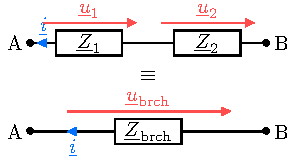
\includegraphics[height=3cm, draft=true]{zserie}
			      }{%
				      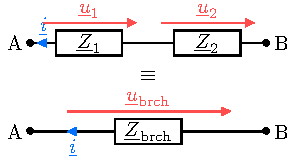
\includegraphics[height=3cm]{zserie}
			      }%
			      \captionof{figure}{Association série \protect\pt{1}}
		      \end{center}
		      \psw{%
			      \[
				      \Iu \stm{=} \frac{\Uu\ind{brch}}{\Zu\ind{brch}} = \frac{\Uu_k}{\Zu_k}
				      \Lra
				      \boxed{
					      \Uu_k \stm{=} \frac{\Zu_k}{\Zu\ind{brch}}\Uu\ind{brch}
				      }%
			      \]
		      }%
		      \tcblower
		      \begin{center}
			      \sswitch{%
				      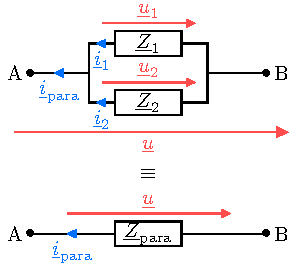
\includegraphics[height=3cm, draft=true]{zpara}
			      }{%
				      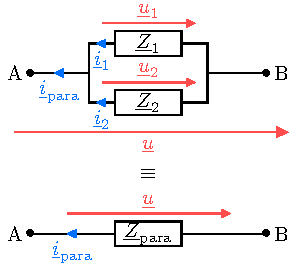
\includegraphics[height=3cm]{zpara}
			      }%
			      \captionof{figure}{Association parallèle \protect\pt{1}}
		      \end{center}
		      \psw{%
			      \[
				      \Uu \stm{=} \Zu\ind{para}\Iu\ind{para} = \Zu_1\Iu_1
				      \Lra
				      \boxed{
					      \Iu_k \stm{=} \frac{\Zu\ind{para}}{\Zu_k}\Iu\ind{para}
				      }%
			      \]
		      }%
	      \end{isd}
	\item[n]{9}%
	      ~
	      \smallbreak
	      \vspace{-25pt}
	      \begin{isd}[righthand ratio=.25, interior hidden, sidebyside align=top]
		      On étudie un circuit RLC série, soumis à une tension sinusoïdale
		      $e(t) = E_0 \cos(\wt)$. \textbf{Représenter le circuit} en complexes,
		      puis déterminer l'\textbf{amplitude complexe} $\Iu$ et la mettre sous
		      la forme $\Iu = \frac{E_0/R}{1+\jj Q \pa{x-\frac{1}{x}}}$, où $x =
			      \w/\w_0$ est la pulsation réduite, et $\w_0$ et $Q$ des constantes
		      \textbf{à identifier} et exprimer en fonction de $R$, $L$ et $C$.
		      Donner son \textbf{amplitude réelle}. Déterminer sa \textbf{pulsation
			      de résonance}.
		      \tcblower
		      \begin{center}
			      \sswitch{%
				      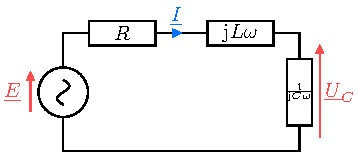
\includegraphics[width=\linewidth, draft=true]{rlc_cplx}
			      }{%
				      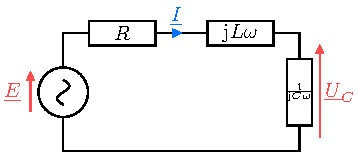
\includegraphics[width=\linewidth]{rlc_cplx}
			      }%
			      \captionof{figure}{Circuit RLC \protect\pt{1}}
		      \end{center}
		      \vspace{-15pt}
	      \end{isd}
	      \smallbreak
	      \noindent
	      \begin{isd}[sidebyside align=top]
		      \psw{%
			      \begin{DispWithArrows*}[fleqn, mathindent=0pt]
				      E_0 & \stm{=}
				      \bigg( R + \jlw + \frac{1}{\jcw} \bigg)\Iu
				      \Arrow{Isole\\$1/\jj = -\jj$}
				      \\\Lra
				      \Iu & =
				      \frac{E_0}{R + \jj \left( L\w - \dfrac{1}{C\w} \right)}
				      \Arrow{Forme\\canonique}
				      \\\Lra
				      \Iu & \stm{=} \frac{E_0/R
				      }{
					      1 + \jj \bigg(
					      \underbracket[1pt]{\dfrac{L}{R}}_{\mathclap{=
							      \frac{Q}{\w_0}\pt{1}}}\w
					      -
					      \underbracket[1pt]{\dfrac{1}{RC}}_{\mathclap{= Q\w_0}}
					      \dfrac{1}{\w}
					      \bigg)
				      }
				      \\\Lra
				      \frac{\frac{1}{RC}}{\frac{L}{R}} =
				      \frac{Q\w_0}{\frac{Q}{\w_0}}
				      \quad & \stm{\text{et}} \quad
				      \frac{L}{R} \times \frac{1}{RC} = Q^2
			      \end{DispWithArrows*}
		      }%
		      \tcblower
		      \psw{%
			      \begin{align*}
				      % \Lra
				      % \frac{\frac{1}{RC}}{\frac{L}{R}} =
				      % \frac{Q\w_0}{\frac{Q}{\w_0}}
				      % \quad & \stm{\text{et}} \quad
				      % \frac{L}{R} \times \frac{1}{RC} = Q^2
				      % \\\Lra
				      % \w_0{}^2 = \frac{1}{LC}
				      % \quad & \text{et} \quad
				      % Q^2 = \frac{1}{R^2} \frac{L}{C}
				      \Lra
				      \boxed{\w_0 = \frac{1}{\sqrt{LC}}}
				      \quad & \stm{\text{et}} \quad
				      \boxed{Q = \frac{1}{R}\sqrt{\frac{L}{C}}}
				      \\\Ra
				      \boxed{\Iu = \frac{E_0/R}{1+\jj Q \pa{x-\frac{1}{x}}}}
				      \quad & \stm{\text{et}} \quad
				      \boxed{I = \frac{E_0/R}{\sqrt{1 + Q^2 \pa{x-\frac{1}{x}}^2}}}
				      \\\Ra
				      I(x_r) \stm{=} I_{\max}
				            & \Lra
				      1 + \underbracket[1pt]{Q^2\left( x_r - \frac{1}{x_r} \right)^2}_{\geq 0}
				      \quad \text{minimal}
				      \\\Lra
				      Q^2\left( x_r - \frac{1}{x_r} \right)^2 = 0
				            & \Lra
				      x_r = \frac{1}{x_r}
				      \\\Lra
				      \boxed{x_r = 1}
				      \quad & \text{ou} \quad
				      \boxed{\w_r = \w_0} \quad \pt{1}
			      \end{align*}
		      }%
	      \end{isd}
	      % \vspace*{-30pt}
	      \ifstudent{
		      \begin{tikzpicture}[remember picture, overlay]
			      \node[anchor=north west, align=left]
			      at ([shift={(1.4cm,0)}]current page.north west)
			      {\\[5pt]\Large\bfseries \textsc{Nom}~:\\[10pt]\Large\bfseries
				      Prénom~:};
			      \node[anchor=north east, align=right]
			      at ([shift={(-1.5cm,-17pt)}]current page.north east)
			      {\Large\bfseries Note~:\hspace{1cm}/20};
		      \end{tikzpicture}
	      }%
\end{enumerate}
\end{document}
